% Chapter 2

\chapter{Path algorithms} % Main chapter title

\label{Chapter6} % For referencing the chapter elsewhere, use \ref{Chapter1} 

\lhead{Chapter 6. \emph{Path algorithms}} % This is for the header on each page - perhaps a shortened title

%----------------------------------------------------------------------------------------
Finding the shortest path is one of the main problems in graph theory. It is a problem of finding a path between two nodes, where the sum of edge weights must be minimized. Graph can be undirected, directed or mixed.
\par The analogy with road maps can be clearly seen, where nodes correspond to intersections and road segments to edges on the graph. To properly represent one way streets we use directed graph. The weight of each edge can be interpreted as a length of each road segment.
\par There are numerous algorithms that are able to found the shortest path. After initial research we narrowed the possible algorithms to:
\begin{itemize}
\item Dijkstra's algorithm
\item A* search algorithm
\item Bellman - Ford algorithm
\item Floyd - Warshall algorithm
\end{itemize}
From the user requirement analysis (segment \ref{user_req}) we were able to identify the three main user requests involving path algorithms:
\begin{itemize}
\item Find shortest path from point A to B (by foot or by car);
\item Find the shortest way to all POIs of a certain category in a radius from point A (by foot or by car);
\item Construct an itinerary from point A to B with visiting POIs in between (with max distance limit);
\end{itemize}

From identified requirements, we can see that all of our path finding problems are actually problems of finding paths between points A and B. This are so-called \textbf{single-pair shortest path problems}. Analysing the algorithms listed above we determined that:
\begin{itemize}
\item Floyd - Warshall algorithm finds shortest paths between every pair of nodes in the graph;
\item Dijkstra and Bellman - Ford algorithms find the shortest paths between source node and all other nodes on the graph (Bellman - Ford also permits negative weights);
\item A* algorithm finds the shortest path between the source and target node. 
\end{itemize}

All of the above algorithms encapsulate the result which we need, but differing in how many unnecessary paths are also calculated. This subsequently mean longer calculation times, which we want to avoid. For this reasons we chose \textbf{A* algorithm} for our path finding problems.

\section{A*}
A* algorithm is one of the most popular path finding algorithms. Its ability to combine the benefits of Dijkstra's algorithm (favouring nodes close to the start node) and Best-First-Search algorithms (favouring nodes close to the target node) makes it efficient and accurate. 
\subsection{Process}
Algorithm works by traversing the graph node by node till it reaches the end node. At every step node with the lowest cost $(f(x))$ is selected. Calculation of the cost is what selected sets A* apart from other greedy best-first search algorithms. Cost is calculated as a weighted sum of:
\begin{itemize}
\item $g(n) - $\textit{exact cost} of the path from the starting point,
\item $h(n) - $\textit{heuristic estimated cost}.
\end{itemize}
Heuristics are used to control the A*'s behaviour. If $h(n)=0$ only distance from the start matters and we have 
normal Dijkstra algorithm. Because we do not know distance from node to end target, as we haven't traversed it yet, we have to estimate it. It is important not to overestimate the distance, as this can cause the algorithm to not found the shortest path. We decided to use air distance as a heuristic, as this guarantees that the actual distance will be equal or greater than that, so we never over-estimate it.





\subsection{Data format}
OpenStreetMap data consists of four core elements:
\begin{itemize}
\item \textbf{Nodes} - basic point of location with longitude and latitude information. They can be used to mark a single point (POI) or in a list of nodes (way, relation);
\item \textbf{Ways} - ordered list of nodes, representing a street or an area like a lake, forest etc.;
\item \textbf{Relations} - ordered list of nodes and ways which can be in a relation (many different roads can be part of a long motorway);
\item \textbf{Tags} - key-value pairs which are used to store information about different objects (nodes, ways, relations).
\end{itemize}
Figure \ref{fig:Osm_flow} shows the difference between different core elements
\begin{figure}[h]
\centering
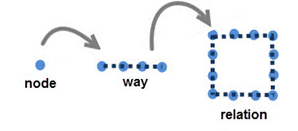
\includegraphics{../pictures/osm_flow.png}
\caption{Representation of basic OSM elements (image taken from \cite{osm_2})}
\label{fig:Osm_flow}
\end{figure}

\section{Points of Interest (POI)}
One of the main requirements for our application is to enable user to search using different points of interest. For acquisition of this points, all of the groups again collaborated, each marking all the points in one part of Le Creusot. For each point we decided to acquire:
\begin{itemize}
\item name;
\item location;
\item address;
\item photo.
\end{itemize}
In the end we also categorized all the points into 26 different categories. 
